\documentclass[12pt,twosides]{extarticle}
\usepackage{jmlda, amsmath, amssymb}
\usepackage{hyperref}
\usepackage{graphicx}
%\NOREVIEWERNOTES

\usepackage{wrapfig}
\usepackage{subfloat}
\usepackage{caption}
\usepackage{multirow}
\newcolumntype{M}[1]{>{\centering\arraybackslash}m{#1}}

\graphicspath{{../pics/}}
%\epstopdfDeclareGraphicsRule{.pdf}{png}{.png}{convert #1 \OutputFile}
%\DeclareGraphicsExtensions{.png,.pdf}
\newtheorem{Th}{Theorem}
%\newtheorem{Def}{Definition}

\title
[under review]
{Spectral graph theory for quality assessment of protein structures
	(Protein model quality assessment using Graph Convolutional Networks based on spectral graph theory)}
\author
[Severilov~P.A.] 
{Pavel Severilov$^1$, Vadim Strijov$^1$} 
% [] список авторов, выводимый в заголовок; не нужен, если он не отличается от основного
%\thanks
%{Научный руководитель:  В.В. Стрижов
%}
\email
{severilov.pa@phystech.edu}
\organization
{$^1$Moscow Institute of Physics and Technology, Russia}
\abstract
{This paper investigates the problem of protein structure quality assessement. The problem is the regression of the modeled protein structures on the value of proximity $\text{CAD}_\text{score}$ between it and the target protein structure. This paper introduce a graphical approach to the problem in combination with the convolution transformation. It analyzes the spectrum of graph convolution and apply graph convolutional neural networks to the protein structure quality assessment problem. The authors propose a regression model and carry out experiments to test it on the data from the CASP competitions. Each molecule from the data represents three-dimensional coordinates and chemical properties of protein atoms. Thus, graphical representations of the data are built. The quality of the proposed model is comparable to the alternative models that give the best quality for the problem.
	
	\bigskip
	\textbf{Keywords}:~\emph{protein structures, graphs, graph convolutions, graph neural networks, convolutional neural networks, spectral analysis}.}


\begin{document}
	\maketitle
	%\linenumbers
	
\section{Introduction}

Proteins are the most universal macromolecules in living systems. They perform essential functions in various biological processes~\cite{berg2002biochemistry}. The shape of a protein structure determines functions it performs~\cite{berg2002biochemistry}. Understanding protein structures and their functions is essential for medical, pharmaceutical and genetic research~\cite{Baldassarre2019GraphQAPM}. Solving the problem of determining in which \textit{target structure} will fold a sequence of amino acids in a protein takes a lot of time and resources.

Every two years the Critical Assessment of Protein Structure Prediction (CASP~\cite{CASP}) competitions are held to solve the protein structure prediction problem. The computational methods, which solve it consist of two stages: modeling the structure of a protein from their amino acid sequences and assessing the quality of prediction. This work develops only the second stage. Prediction quality is understood as the value of the proximity of \textit{modeled} and target structures (for example, metrics $\text{CAD}_\text{score}$~\cite{Olechnovic2013CADscoreAN}, LDDT~\cite{Mariani2013lDDTAL}, GDT~\cite{GDT}). It is computationally expensive calculating these metrics directly, so this problem is considered as an individual task.
\begin{figure}[H]
	\centering
	\subfloat[Target T0861]{\label{fig:edge-a}
		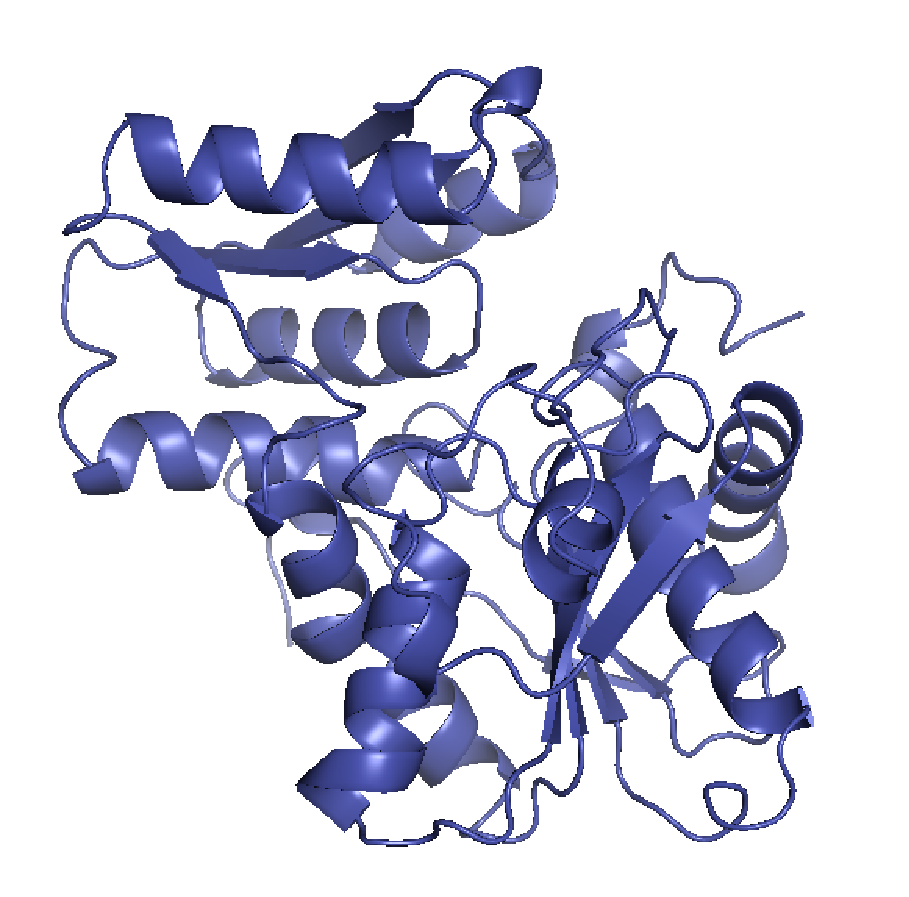
\includegraphics[scale=0.24]{target_T0861.pdf}}
	\subfloat[Modeled Atome2\_CBS\_TS4]{\label{fig:edge-b}
		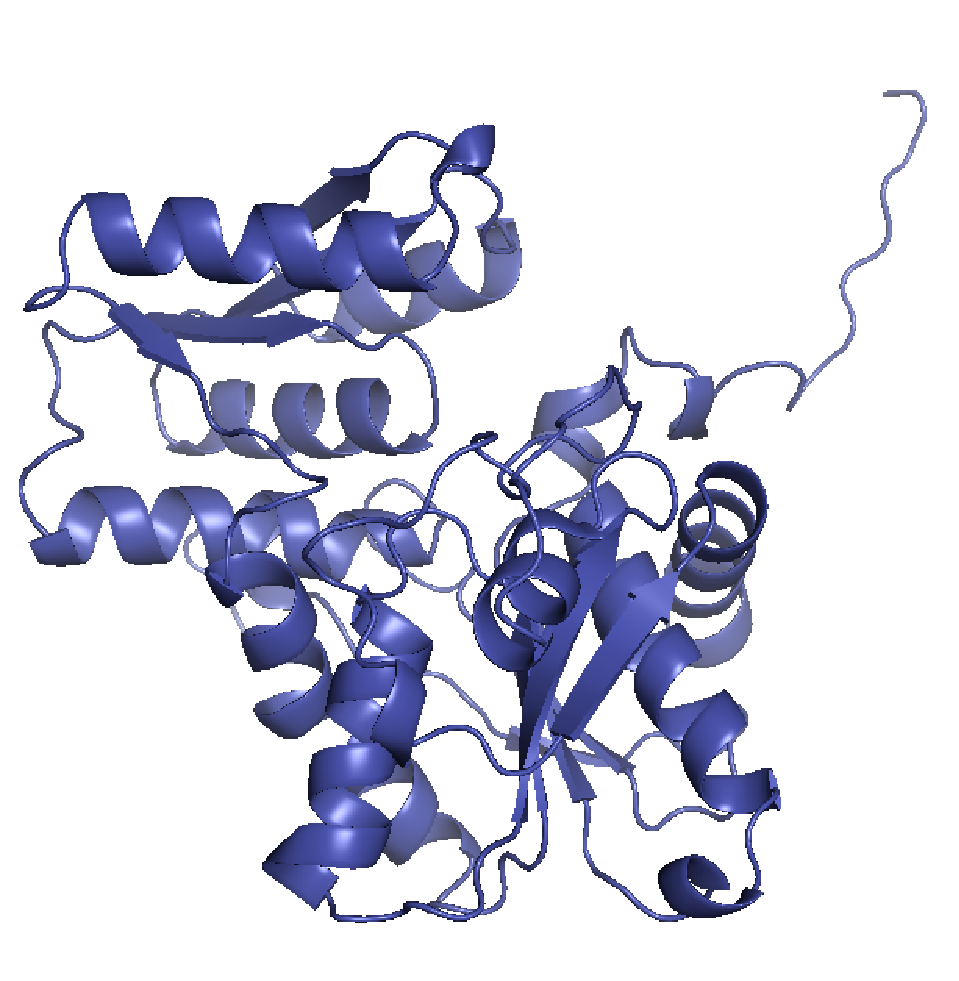
\includegraphics[scale=0.24]{model_T0861.pdf}}
	\captionof{figure}{Example of target and model protein structures}
	\label{fig:edge}
\end{figure}
The protein structure consists of one or more chains of smaller molecules~-- amino acid residues. The sequence of residues S=$\{a_i\}_{i = 1}^N $ represents its primary structure, where $a_i$ is one of 22 types of amino acids. The interactions between neighboring residues and the environment determine how the chain folds into complex structures that represent the secondary structure and tertiary structure of the protein~\cite{Baldassarre2019GraphQAPM}.

Therefore, it is necessary to take into account both spatial information about atoms, tertiary structure, and features in the form of sequences, the primary structure of the protein for the tasks of predicting and assessing the quality of protein structures. In~\cite{HurtadoQA, AngularQA} the authors used LSTM or 1D-CNN  to assess the quality of protein structures prediction. These methods represent proteins as a sequence with spatial features. In~\cite{3DCNN, 10.1093/bioinformatics/btz122},  the authors predict the quality of protein structure using 3D-CNN, but the primary structure of the protein is not taken into account. These papers do not take into account both the primary and tertiary structures of the proteins.  We can take into account both amino acid sequences and spatial, geometric structures of proteins by using the graph representation.

\begin{figure}[t]
	\centering
	%\includegraphics[width=1.02\textwidth]{experiment.pdf}
	\includegraphics[width=0.91\textwidth]{main_slide_eng.pdf}
	\caption{Protein Structure Quality Assessment diagram}
	\label{fig:experiment}
\end{figure}
The work~\cite{Baldassarre2019GraphQAPM} is the only one where authors use a graph representation of the protein structure to solve the problem of protein structure model quality assessement. The authors used graph neural networks based on the algorithm described in~\cite{Battaglia2018RelationalIB}. These networks show results that are superior to other state of the art methods. The model from~\cite{Baldassarre2019GraphQAPM} does not use convolutions. The main results in the protein quality assessement problem rely on convolutional neural networks (CNNs)~\cite{10.1093/bioinformatics/btz122}. In our paper, we associate the success of convolutional neural networks and graph representation of proteins to solve the protein quality assessment problem.

Figure~\ref{fig:experiment} shows a diagram of solving the protein quality assessment problem using CNNs and graph representation of proteins. We define convolution on graphs by the methods of spectral graph theory. Then we analize its spectrum. A graph convolutional neural network model for the quality assessing of protein structure prediction was built on the basis of the obtained graph convolution transform. The data for the experiments were taken from the CASP competitions of previous years. Each molecule from the data is presented in the form of information about atoms and their spatial location for target and modeled protein structures. We construct graph representation of each modeled structure based on this data -- the coordinate matrix $ \mathbf{X} $ and the adjacency matrix $\mathbf{A}$.


%-----------------------------------------------------------------------------------------------------
\section{Problem statement for quality assessment of protein structure}

There given a sample set $$\mathfrak{D} = \left\{\mathbf{x}_i, {y}_i\right\}_{i=1}^m,$$ where $\mathbf{x}_i\in \mathbb{R}^{n_i\times 3}$ are molecules. Each vector describes a set of three-dimensional coordinates of all its $n_i$ atoms, ${y}_i \in \mathbb{R}$ is a proximity assessment of modeled and target protein structures. The proximity assessment is measured by various metrics: $\text{CAD}_\text{score}$~\cite{Olechnovic2013CADscoreAN}, LDDT~\cite{Mariani2013lDDTAL}, GDT~\cite{GDT}. In this paper, $\text{CAD}_\text{score}$ is selected. 

%-----------------------------------------------------------------------------------------------------
\subsection{Estimation of CAD score~\cite{Olechnovic2013CADscoreAN}}
%\begin{wrapfigure}{r}{0.32\textwidth}
%	\centering
%	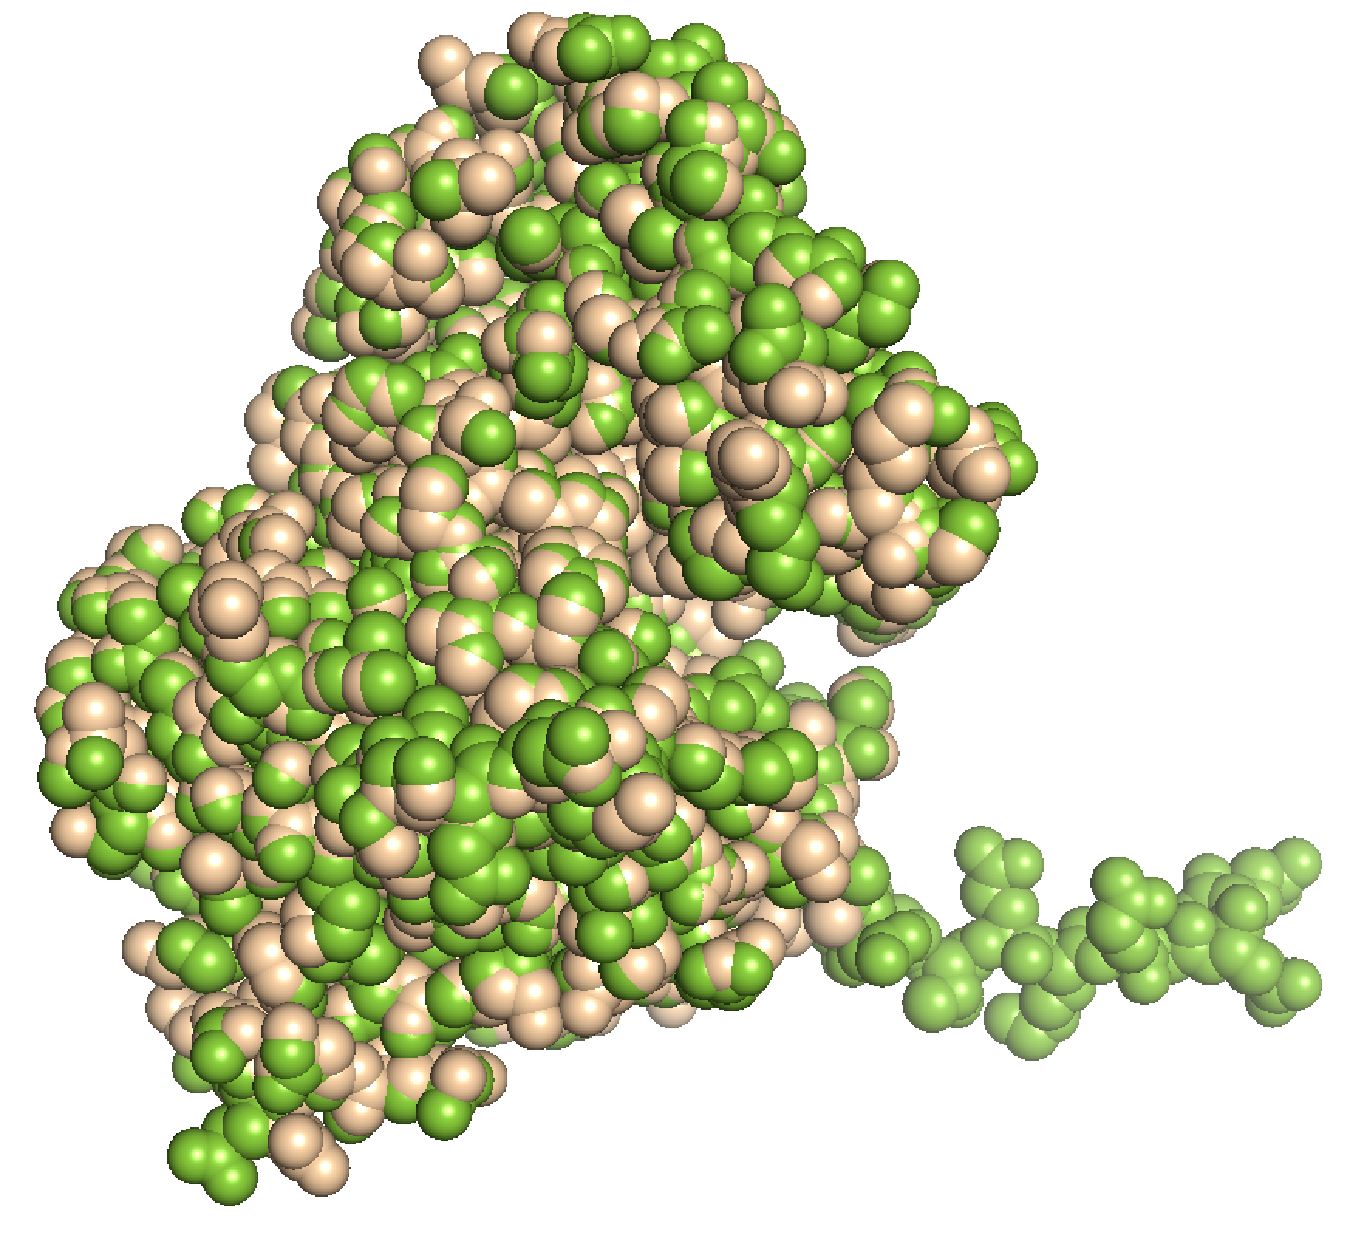
\includegraphics[width=0.3\textwidth]{T0861_Atome2_CBS_TS4.pdf}
%	\caption{Пересечение реальной и смоделированной структур}
%	\label{CAD_example}
%\end{wrapfigure}

$P$ Denotes the set of all pairs of elements of the amino acid sequence (residues) $(i, j)$ that have a nonzero contact area $N_{(i, j)}$ in the target structure. Then, for each pair of residues $ (i, j) \in P $ we calculate the contact area $ M_{(i, j)} $ of the modeled structure.

For each pair of residues $ (i, j) \in P $, the difference in the contact areas $ \mathrm{CAD}_{(i, j)}$ is determined as the absolute difference in the contact areas between the residues $ i $ and $ j $ in the target $ N $ and the modeled structure $ M $:
$$\mathrm{CAD}_{(i, j)}=\left|N_{(i, j)}-M_{(i, j)}\right|.$$

We take a bounded $\mathrm{CAD}_{(i, j)}$ for computational stability: $\mathrm{CAD}_{(i, j)}^{\text {bounded}}=\min \left(\mathrm{CAD}_{(i, j)}, N_{(i, j)}\right)$. Thus, $\text{CAD}_\text{score}$ for the entire structure is defined as
\begin{align}
\mathrm{CAD}_\text{score}=1-\cfrac{\sum_{(i, j) \in P} \mathrm{CAD}_{(i, j)}^{\text {bounded }}}{\sum_{(i, j) \in P} N_{(i, j)}}.
\label{CAD_score}
\end{align}

Figure~\ref{CAD_example} shows an example of the intersection of the target structure T0861 (yellow) and its modeled structure Atome2\_CBS\_TS4 (green) with $\mathrm{CAD}_\text{score}=0.829$.
\begin{figure}[h]
	\centering
	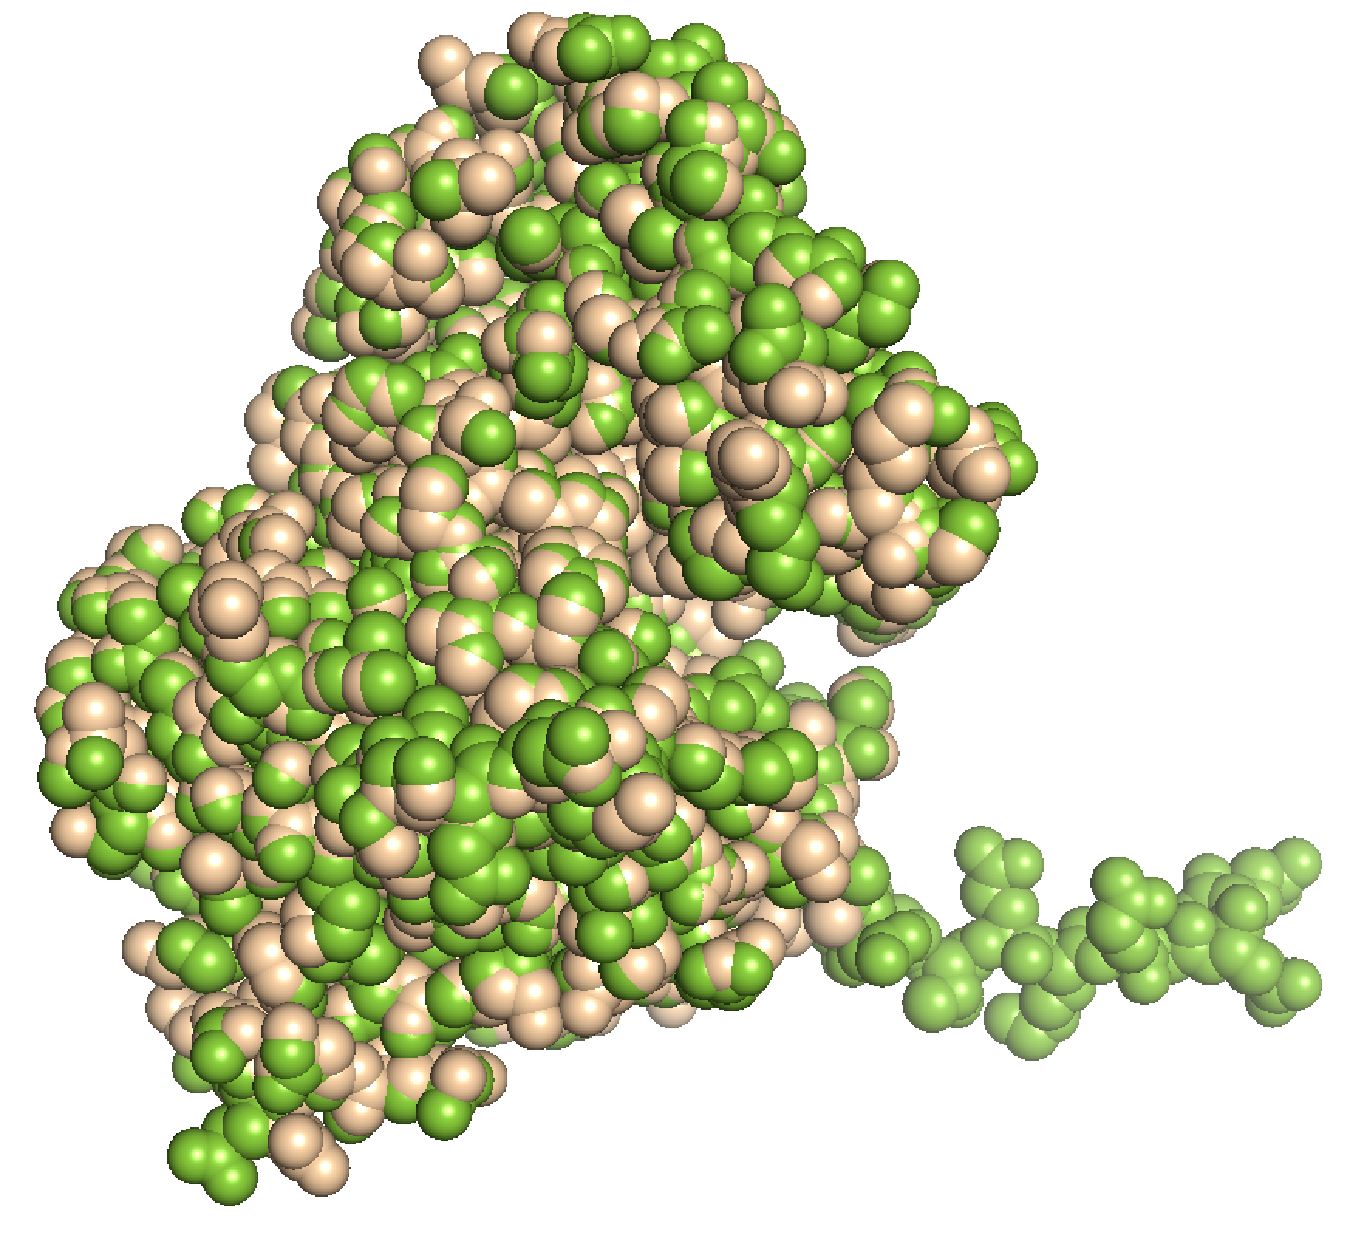
\includegraphics[width=0.3\textwidth]{T0861_Atome2_CBS_TS4.pdf}
	\caption{Intersection of target and modeled structures}
	\label{CAD_example}
\end{figure}
%-----------------------------------------------------------------------------------------------------
\subsection{Regression of protein structures on~$\text{CAD}_\text{score}$}

Denote $\mathbf{X} = \bigcup_{i=1}^m \mathbf{x}_i$. A set of parametric models which maps $\mathbf{X}$ to a vector of $\text{CAD}_\text{score}$ predictions $\hat{\mathbf{y}} = \mathbf{f} (\mathbf{X},\mathbf{w}) \in \mathbb{R}^{m}$:
\begin{align}
\mathfrak{F} = \{\mathbf{f}_k\colon(\mathbf{w}, \mathbf{X})\to  \mathbf{\hat{y}}\mid k \in \mathfrak{K}\},
\label{params_models}
\end{align} 
where $\mathbf{w} \in \mathbb{W}$ are the model parameters. The models are taken from the class of graph convolutional neural networks.

This paper solves the regression problem for predicting the numerical value of $\text{CAD}_\text{score}$  $y_i$ from the modeled protein structure $\mathbf{x}_i$.

The model parameters $\mathbf{w}\in \mathbb{W}$ minimize the error function. The error function is defined as
\[\mathfrak{L}(\mathbf{y}, \mathbf{X}, \mathbf{w}) =\left\lVert \hat{\mathbf{y}} - \mathbf{y} \right\rVert^{2}_2,\]
where $\mathbf{\hat{y}} = \mathbf{f} (\mathbf{X},\mathbf{w})$ is the $\text{CAD}_\text{score}$ predicted by the model $\mathbf{f}$, $\mathbf{y}$ is the ground-truth $\text{CAD}_\text{score}$ given in the sample set $\mathfrak{D}$.
Thus, one has to solve the optimization problem
$$\textbf{w}^* = \underset{\mathbf{w}\in\mathbb{W}}{\text{argmin}}(\mathfrak{L}(\textbf{w})).$$

We analyze Pearson ($R$) and Spearman ($\rho$) correlation coefficients~\cite{3DCNN, Baldassarre2019GraphQAPM, 10.1093/bioinformatics/btz122}. It helps to understand how close the modeled structure is to the target structure based on the predictions of the regression model and the ground truth values. We calculate the Pearson ($R^\text{target}$) and Spearman ($\rho^\text{target}$) correlation coefficients for each target structure between the ground truth and predicted $\text{CAD}_\text{score}$ for modeled protein structure. Then the correlation coefficients are averaged over all $T$ target structures.
Denote $\mathbf{y}_i \in \mathbf{R}^{m_i}$ and $\mathbf{\hat{y}}_i \in \mathbf{R}^{m_i}$, respectively, the vector of ground truth values and the vector of $\text{CAD}_\text{score}$ predictions for modeled protein structures corresponding to the target structure $i$. Here $m_i$ is the amount of modeled structures for the $i$-th target structure. Then the correlation coefficients are presented as
\begin{align}
R = R\left(\mathbf{y}, \hat{\mathbf{y}}\right) = \frac{1}{T} \sum_{i=1}^{T} R^\text{target}_i=\frac{1}{T} \sum_{i=1}^{T} \text{PEARSON} \left(\mathbf{y}_i,\hat{\mathbf{y}}_i\right) \label{pearson}
\\ 
\rho= \rho\left(\mathbf{y}, \hat{\mathbf{y}}\right) = \frac{1}{T} \sum_{i=1}^{T} \rho^\text{target}_i = \frac{1}{T} \sum_{i=1}^{T} \text{SPEARMAN} \left(\mathbf{y}_i,\hat{\mathbf{y}}_i\right)
 \label{spearman}
\end{align}
Here $\text{PEARSON} (\cdot, \cdot)$ and $\text{SPEARMAN} (\cdot, \cdot)$ are Pearson and Spearman correlations, respectively:
\[\text{PEARSON}\left(\mathbf{y}_i,\hat{\mathbf{y}}_i\right) = \frac{\sum_{l=1}^{m_i}\left(\mathbf{y}_{i l}-\bar{\mathbf{y}}_{i}\right)\left( \hat{\mathbf{y}}_{i l}-\bar{ \hat{\mathbf{y}}}_{i}\right)}{\sqrt{\sum_{l=1}^{m_i}\left( \mathbf{y}_{i l}-\bar{ \mathbf{y}}_{i}\right)^{2} \sum_{l=1}^{m_i}\left( \hat{\mathbf{y}}_{i l}-\bar{ \hat{\mathbf{y}}}_{i}\right)^{2}}}\]

\[ \text{SPEARMAN} \left(\mathbf{y}_i,\hat{\mathbf{y}}_i\right)=\frac{\sum_{l=1}^{m_i}\left(\text{rank}\left(
	\mathbf{y}_{i l}\right)-\frac{m_i+1}{2}\right)\left(\text{rank}
	\left( \hat{\mathbf{y}}_{i l}\right)-\frac{m_i+1}{2}\right)}{\frac{1}{12}\left(m_i^{3}-m_i\right)}
\]

%-----------------------------------------------------------------------------------------------------
\subsection{Making the adjacency matrices}
Protein data does not contain information about the connections between atoms. Therefore, we calculate adjacency matrices $\textbf{A}$ for modeled protein structures from the CASP data according to the following rules:

\begin{itemize}
	\item hydrogen does not connect with hydrogen,
	\item an atom does not connect with hydrogen if the distance between them is at least $1.21$\AA,
	\item atoms that are far away in the sequence do not connect (residue numbers differ by more than 1),
	\item atoms that create disulfide bonds do not connect,
	\item atoms are connected, if the distance between them is $r\in \left(r_\text{min}, r_\text{max}\right]$, where $r_\text{min} = 0.01$\AA, $r_\text{max} = \left(0.6\cdot(\rho_\text{atom1}+\rho_\text{atom2})\right)^2$, $\rho_\text{atom}$ -- atomic radius (maximum possible $r_\text{max} = 5.76$ -- at $\rho_\text{atom1} = \rho_\text{atom2} = 2.0$).
\end{itemize}

The maximum possible distance between atoms, at which they can have a connection according to the presented rules for composing the adjacency matrix, is 5.76~\AA. Pairwise distances between atoms in figure~\ref{protein_vis} shows that atoms marked only with the lightest yellow may have connections. Hence, the adjacency matrix is highly sparse.

\begin{figure}[H]
	\centering
	\begin{minipage}[b]{0.49\textwidth}
		\centering
		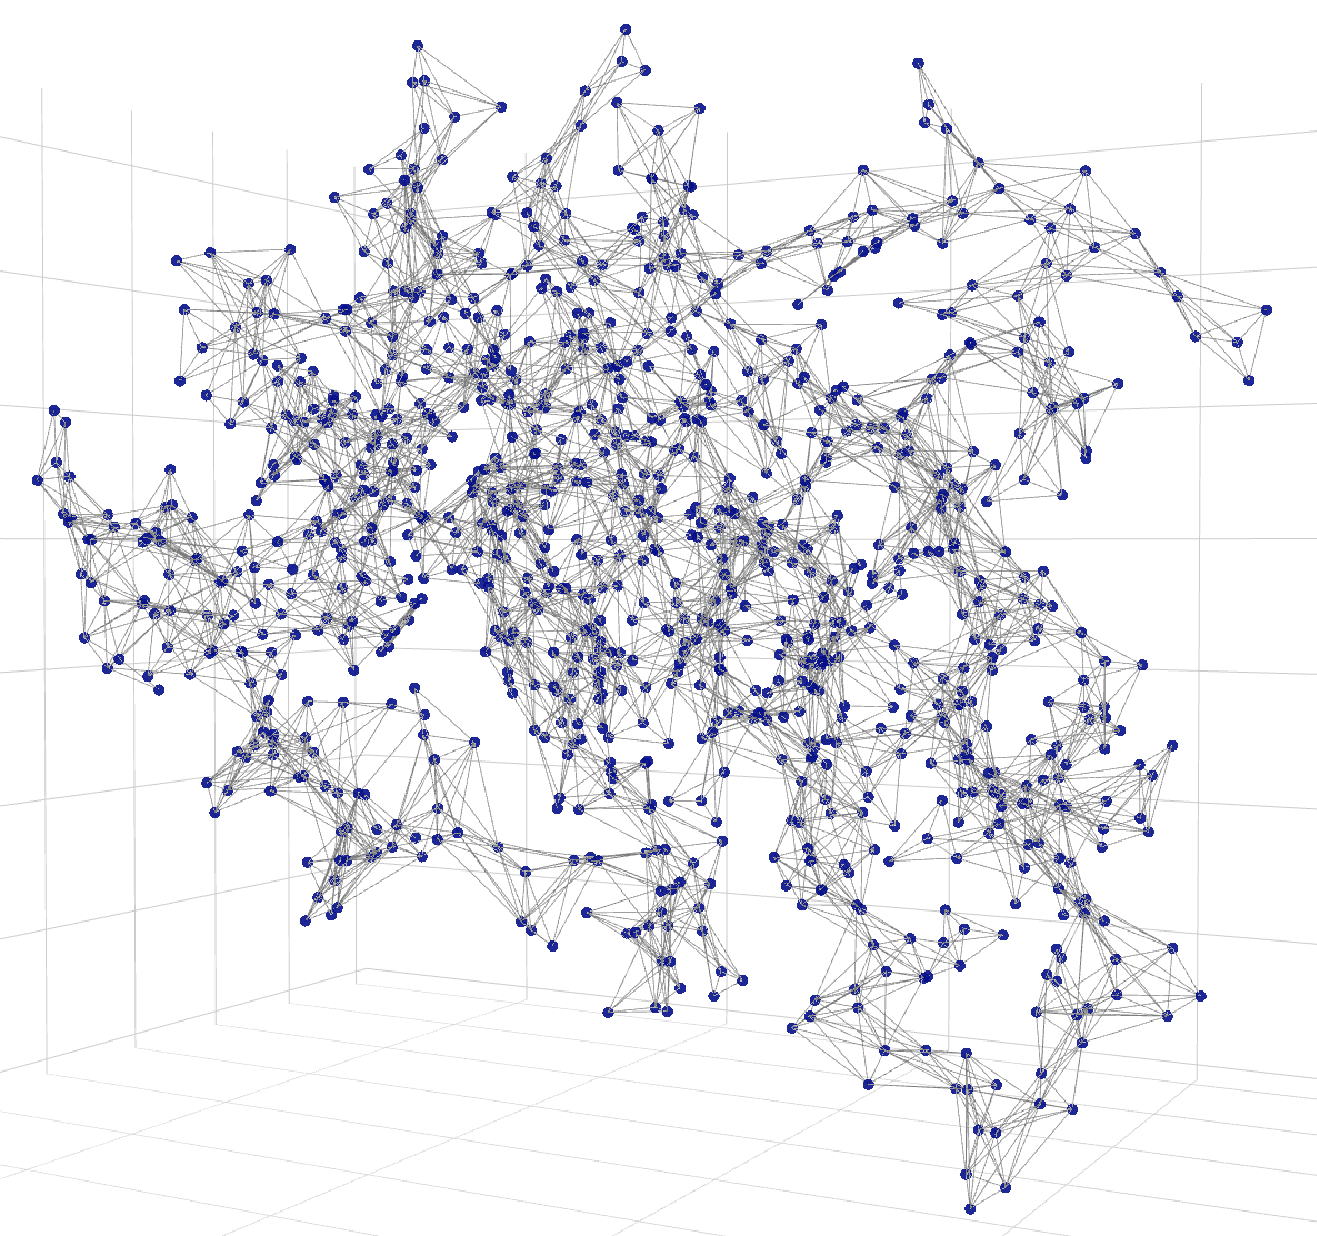
\includegraphics[width=0.99\textwidth]{3d_graph.pdf}
		%	\caption{3D визуализация }
		%	\label{fig:data}
	\end{minipage}
	%\hfill
	\begin{minipage}[b]{0.49\textwidth}
		\centering
		\includegraphics[width=0.99\textwidth]{pairwise_eng.pdf}
		%	\caption{Попарные расстояния между элементами белка}
		%	\label{fig:data}
	\end{minipage}
	\caption{Three-dimensional representation using coordinates $\textbf{X}$ and the resulting adjacency matrix $\textbf{A}$; pairwise distances between atoms of the modeled structure BAKER-ROSETTASERVER\_TS3 of the target structure T0870 from the CASP12 dataset}
	\label{protein_vis}
\end{figure}


%-----------------------------------------------------------------------------------------------------
\section{Spectral analysis}

It is required to define convolutional filters on graphs to generalize convolutional neural networks to graphs. There are two approaches: spatial and spectral~\cite{DBLP:journals/corr/abs-1901-00596, DBLP:journals/corr/abs-1812-08434}. As shown in~\cite{ae482107de73461787258f805cf8f4ed}, the spatial approach does not have a general mathematical definition of translation on graphs, while the spectral method has a good mathematical foundation. Therefore, the spectral graph theory is considered.

%\subsection{Представление белковых структур в виде графов}
The elements of the amino acid sequence are correspond to nodes, whose connections (edges) describe the spatial relationship between them.

In general case, the graph $\mathbf{G}$ is defined by the set $\mathbf{(V, A)}$, where $\mathbf{V}\in \mathbb{R}^{n \times c}$ defines the nodes of the graph. The adjacency matrix $\mathbf{A}\in \mathbb{R}^{n \times n}$ defines connections between $n$ nodes (edges), where $\mathbf{A}_{ij}$ is the presence of a connection between nodes $i$ and $j$. We define protein structure as graph using this definition of a graph. The features of amino acid sequence elements are correspond to the elements of $\mathbf{V}$. The spatial proximity between elements is corresponds to the adjacency matrix $\mathbf{A}$.

\subsection{Graph convolution transform}

\begin{Def}
	\textit{Graph Laplacian}~\cite{Chung:1997} is a matrix $\mathbf{L}=\mathbf{I}_{n}-\mathbf{D}^{-\frac{1}{2}} \mathbf{A} \mathbf{D}^{-\frac{1}{2}}$, where $\mathbf{A}$ is a graph adjacency matrix $\mathbf{G}$,  $\mathbf{D}$ is a diagonal matrix of node degrees, $\mathbf{D}_{i i}=\sum_{j}\left(\mathbf{A}_{i j}\right)$ and $\mathbf{I}_{n}$ is an identity matrix.
\end{Def}

The matrix $\mathbf{L}$ is real-valued symmetric positive semidefinite, therefore it can be represented as $\mathbf{L}=\mathbf{U} \boldsymbol{\Lambda} \mathbf{U}^{\mathsf{T}} $, where $\mathbf{U}=\left[\mathbf{u}_{1}, \mathbf{u}_{2}, \dots, \mathbf{u}_n\right] \in \mathbb{R}^{n \times n}$ is the matrix of eigenvectors ordered by eigenvalues, $\boldsymbol{\Lambda} \in \mathbb{R}^{n \times n}$ is the diagonal eigenvalue matrix (spectrum), $\boldsymbol{\Lambda}_{i i}=\lambda_{i}$. The Laplacian spectral decomposition allows one to determine the Fourier transform on graphs: its eigenvectors correspond to the Fourier decomposition modes and its eigenvalues correspond to frequencies.

\begin{Def}
	The \textit{Graph Fourier Transform}~\cite{journals/spm/ShumanNFOV13} for a signal $\mathbf{x} \in \mathbb{R}^{n}$ is defined(given) by \[\mathscr{F}(\mathbf{x})=\mathbf{U}^{\mathsf{T}} \mathbf{x} \equiv \hat{\mathbf{x}} \in \mathbb{R}^{n},\] where $\mathbf{x}$ -- vector of features of all vertices. Inverse graph Fourier transform: $\mathscr{F}^{-1}(\hat{\mathbf{x}})=\mathbf{U} \hat{\mathbf{x}}$.
\end{Def}

This transformation is key in defining the graph convolution. It projects the input graph signal onto an orthonormal space, where the basis is formed by the eigenvectors of the graph Laplacian. The elements of the transformed signal  $ \hat{\mathbf{x}}$ are coordinates of the signal in the new space, so the input signal can be represented as $\mathbf{x}=\sum_{i} \hat{x}_{i} \mathbf{u}_{i}$. It is the inverse graph Fourier transform.

\begin{Th}
	\textbf{(Convolution theorem)}~\cite{10.5555/1525499} The Fourier transform of the convolution of two signals is the component-wise product of their Fourier transforms: $$\mathscr{F}\left( \mathbf{f} * \mathbf{g}\right) =\mathscr{F}(\mathbf{f}) \odot \mathscr{F}(\mathbf{g}).$$
	\label{conv_theorem}
\end{Th}

Following from the theorem~\ref{conv_theorem}, the spectral convolution on graphs is defined for the signal $\mathbf{x}$ and the filter $\mathbf{g} \in \mathbb{R}^{n}$ as
\begin{align}
\mathbf{x} * \mathbf{g} &=\mathscr{F}^{-1}(\mathscr{F}(\mathbf{x}) \odot \mathscr{F}(\mathbf{g})) =\mathbf{U}\left(\mathbf{U}^{\mathsf{T}} \mathbf{x} \odot \mathbf{U}^{\mathsf{T}} \mathbf{g}\right) = \mathbf{U g}_{\theta} \mathbf{U}^{\mathsf{T}} \mathbf{x},\label{spec_conv}
\end{align}
where $\mathbf{g}_{\theta} = \text{diag}\left(\mathbf{U}^{\mathsf{T}} \mathbf{g}\right)$ are the spectral filter coefficients.

Spectral methods differ in selection of a filter $\mathbf{g}_{\theta}$. The expression~\eqref{spec_conv} is computationally expensive because the spectral decomposition requires $O\left(n^{3}\right)$ operations and multiplication with eigenvector matrix $\mathbf{U}$  requires $O\left(n^{2}\right)$  operations. Chebyshev Spectral CNN (ChebNet)~\cite{NIPS2016_6081} solves these problems by approximating $\mathbf{g}_{\theta}$ using Chebyshev polynomials $\mathbf{T}_k\mathbf{(x)}$, removing the need to calculate the Laplacian eigenvectors $\mathbf{L}$.

\begin{Def}
	The $k$-th order \textit{Chebyshev polynomials} $\mathbf{T}_k\mathbf{(x)}$ are given by the recurrence relation $ \mathbf{T}_{k}(\mathbf{x})=2 \mathbf{x} \cdot \mathbf{T}_{k-1}(\mathbf{x})-\mathbf{T}_{k-2}(\mathbf{x}), \mathbf{T}_{0}(\mathbf{x})=1, \mathbf{T}_{1}(\mathbf{x})=\mathbf{x}$. The polynomials form an orthogonal basis in $L^{2}\left([-1,1], \cfrac{d x} {\sqrt{1-x^{2}}}\right).$
\end{Def}

Represent $\mathbf{g}_{\theta}$ as
\[\mathbf{g}_{\theta}=\sum_{k=0}^{K} \theta_{k} \mathbf{T}_{k}\mathbf{(\tilde{\Lambda})},	\]
where $\mathbf{\tilde{\Lambda}} = 2 \mathbf{\Lambda} / \lambda_{\max }-\mathbf{I}_{n} \in[-1,1]$, $\lambda_{\max }$ is the maximum eigenvalue $\mathbf{L}$, and notice that
\[
\left(\mathbf{U} \mathbf{\Lambda} \mathbf{U}^{\mathsf{T}}\right)^{k}=\mathbf{U} \mathbf{\Lambda}^{k} \mathbf{U}^{\mathsf{T}}
\]
(the eigenvectors form an orthonormal basis $\mathbf{U}^{\mathsf{T}}\mathbf{U}=\mathbf{I}$). Then get:
\begin{align}
\mathbf{U g}_{\theta} \mathbf{U}^{\mathsf{T}} \mathbf{x}=\mathbf{U}\left(\sum_{i=0}^{K} \theta_{k} \mathbf{T}_{k}(\tilde{\mathbf{\Lambda}})\right) \mathbf{U}^{\mathsf{T}} \mathbf{x} = \sum_{k=0}^{K} \theta_{k} \mathbf{T}_{k}(\tilde{\mathbf{L}}) \mathbf{x},
\label{cheb_appr}
\end{align}
where $\tilde{\mathbf{L}}=2 \mathbf{L} / \lambda_{\max }-\mathbf{I}_{n}$.

Graph Convolutional Network (GCN)~\cite{kipf_semi-supervised_2017} use the first ChebNet approximation. Assuming $\lambda_{\max} \approx 2$ and taking the first 2 terms in the sum ($K=1$), the expression~\eqref{cheb_appr} simplifies to
\begin{align}
\mathbf{x} * \mathbf{g} \approx \tilde{\theta}_{0} \mathbf{x}+\tilde{\theta}_{1}\left(\mathbf{L}-\mathbf{I}_{n}\right) \mathbf{x}=\tilde{\theta}_{0} \mathbf{x}-\tilde{\theta}_{1} \mathbf{D}^{-\frac{1}{2}} \mathbf{A} \mathbf{D}^{-\frac{1}{2}} \mathbf{x}.
\end{align}
Taking $\theta = \tilde{\theta}_0  = -\tilde{\theta}_1$, obtain:
\begin{align}
\mathbf{x} * \mathbf{g}  \approx \theta\left(\mathbf{I}_{n}+\mathbf{D}^{-\frac{1}{2}} \mathbf{A} \mathbf{D}^{-\frac{1}{2}}\right) \mathbf{x}.
\label{conv}
\end{align}
The operator $\left(\mathbf{I}_{n}+\mathbf{D}^{-\frac{1}{2}} \mathbf{A} \mathbf{D}^{-\frac{1}{2}}\right) $ can lead to computational instability and gradient explosion or vanishing, because the eigenvalues of this operator are $\in [0,2]$. The authors of~\cite{kipf_semi-supervised_2017} propose a \textit{renormalization trick} to solve this problem:
\begin{align*}
\mathbf{I}_{n}+\mathbf{D}^{-\frac{1}{2}} \mathbf{A} \mathbf{D}^{-\frac{1}{2}} \rightarrow
\tilde{\mathbf{D}}^{-\frac{1}{2}} \tilde{\mathbf{A}}\tilde{\mathbf{D}}^{-\frac{1}{2}}, 
\text{ где }
\tilde{\mathbf{A}}=\mathbf{A}+\mathbf{I}_{n},~ \tilde{\mathbf{D}}_{i i}=\sum_{j} \tilde{\mathbf{A}}_{i j}.
\end{align*}
There given a graph $\mathbf{G}$ and a matrix $\mathbf{X} \in \mathbb{R}^{n \times c}$ with information about nodes ($n$ is the number of nodes and $c$ is the number of features in each node). Based on~\eqref{conv} and applying the renormalization trick, the graph convolution layer is determined:
\begin{align}
\textbf{U}=\tilde{\mathbf{D}}^{-\frac{1}{2}} \tilde{\mathbf{A}}\tilde{\mathbf{D}}^{-\frac{1}{2}} \mathbf{X} \mathbf{W},
\label{Z_conv}
\end{align}
where $\mathbf{W} \in \mathbb{R}^{c \times t}$ is the convolution parameter matrix with $t$ filters, and $\textbf{U} \in \mathbb{R}^{n \times t}$ is the output matrix. Figure~\ref{fig:convlayer} shows the scheme of a graph convolutional layer.
\begin{figure}[H]
	\centering
	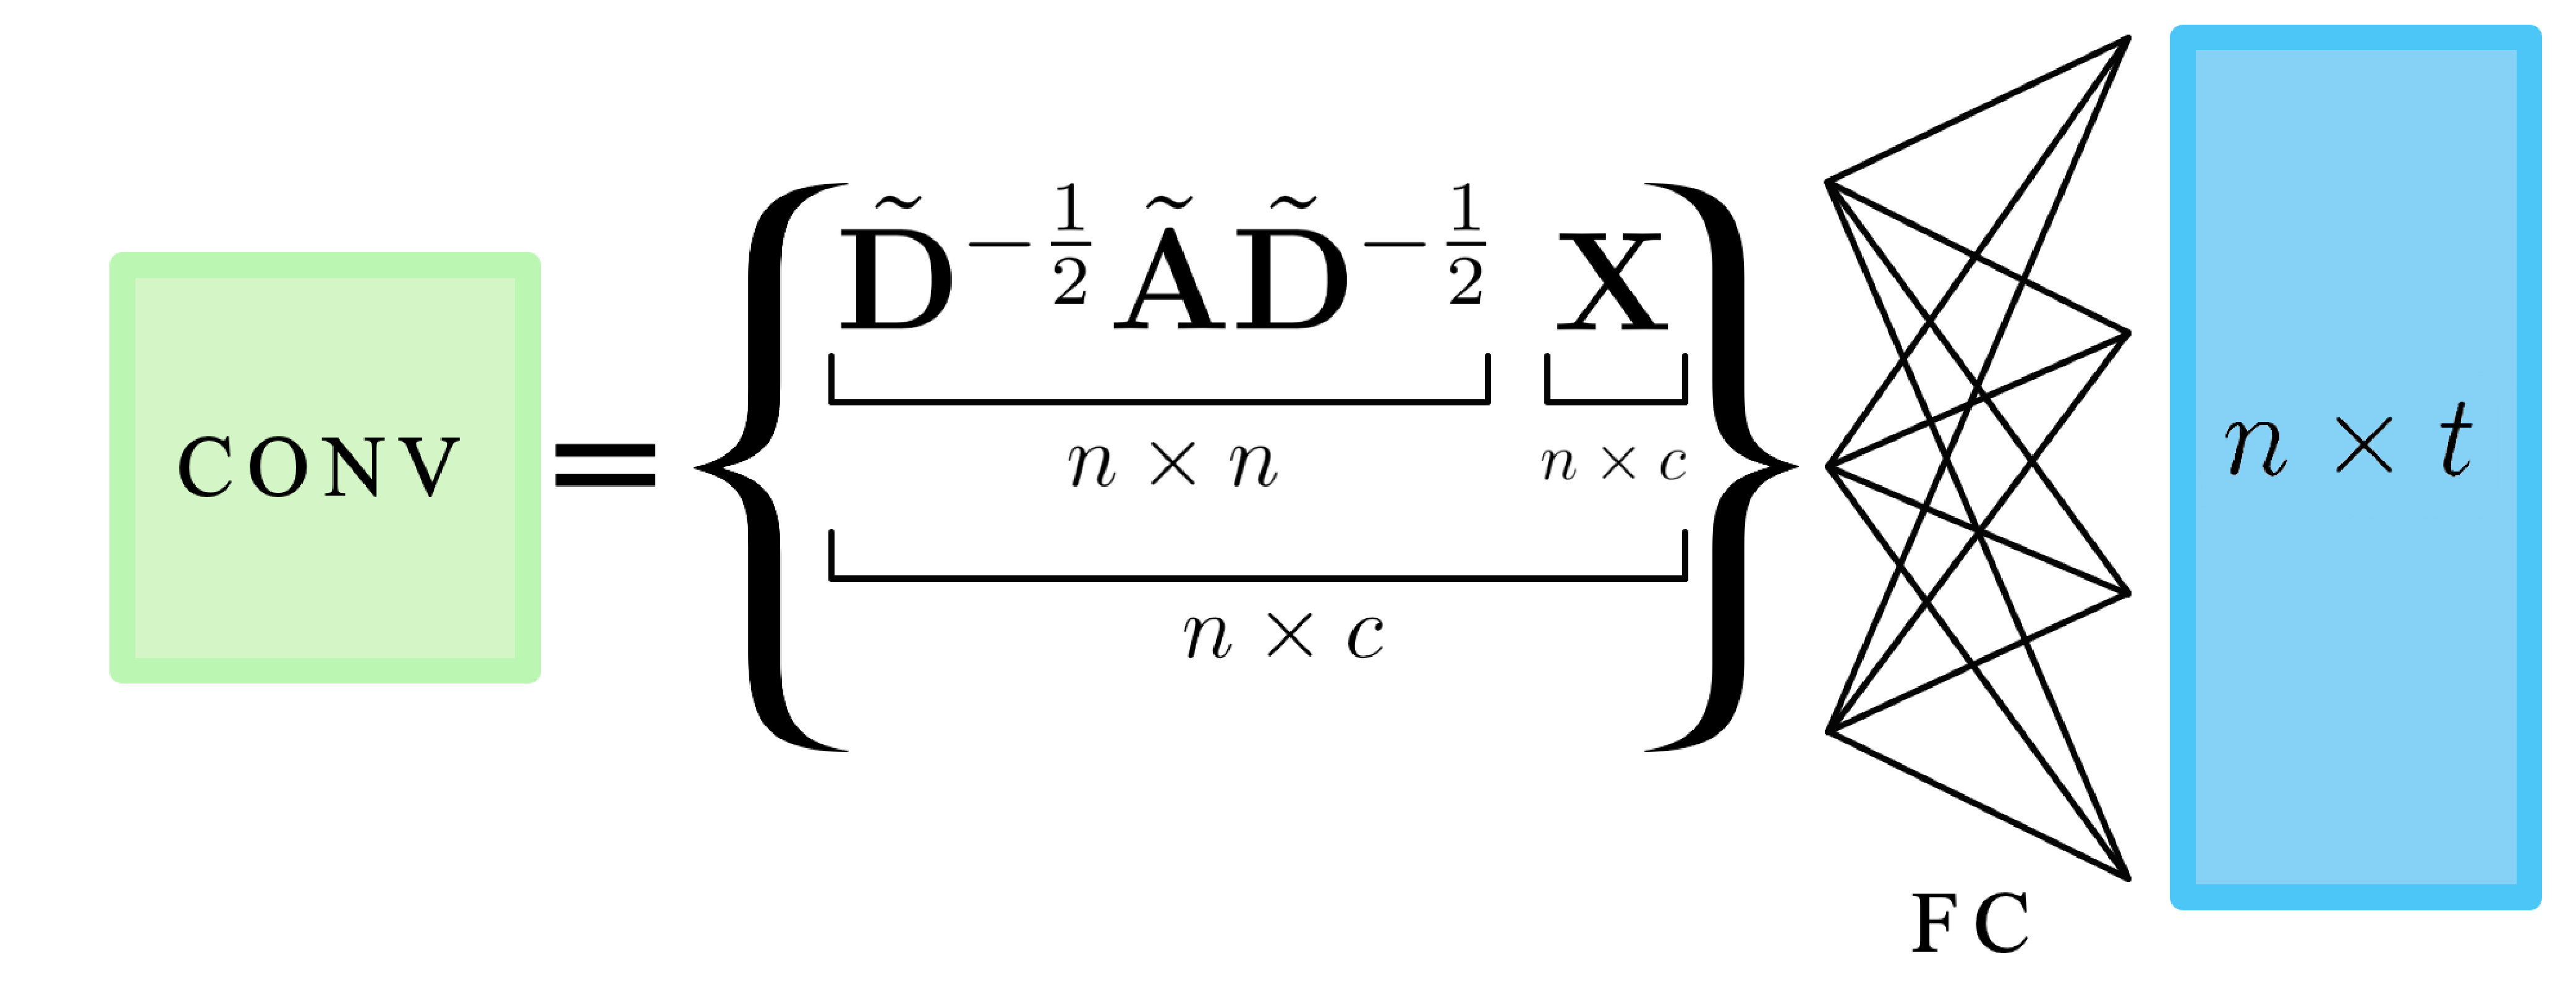
\includegraphics[width=0.55\textwidth]{conv_layer.pdf}
	\caption{A graph convolution scheme with the matrix $\textbf{X}$ of size $ n \times c$, where $\text{t}$ is the number of filters in the convolution, FC is a fully connected layer. The blue rectangle corresponds to the output matrix of size $n\times t$}
	\label{fig:convlayer}
\end{figure}


%-----------------------------------------------------------------------------------------------------
\subsection{Regression model transformation function}
The network architecture is constructed similar to the GCN~\cite{kipf_semi-supervised_2017} model. The expression~\eqref{Z_conv} defines convolutional layers (Fig.~\ref{fig:convlayer}). ReLu is selected as the nonlinear function~$\sigma$.

The network SpectralQA~\eqref{params_models} consists of three convolutional layers, $\text{pool}$ max-pooling over the nodes and a fully connected $\text{FC}$~layer. Last $\text{FC}$~layer is the scalar multiplication with the vector $\mathbf{w}_4$. The convolution parameters $t$ are taken equal to 64, 64, 64, respectively, for the first, second and third convolutional layers. Fig.~\ref{fig:scheme} shows the scheme of the neural network tested in this paper.
\begin{figure}[H]
	\centering
	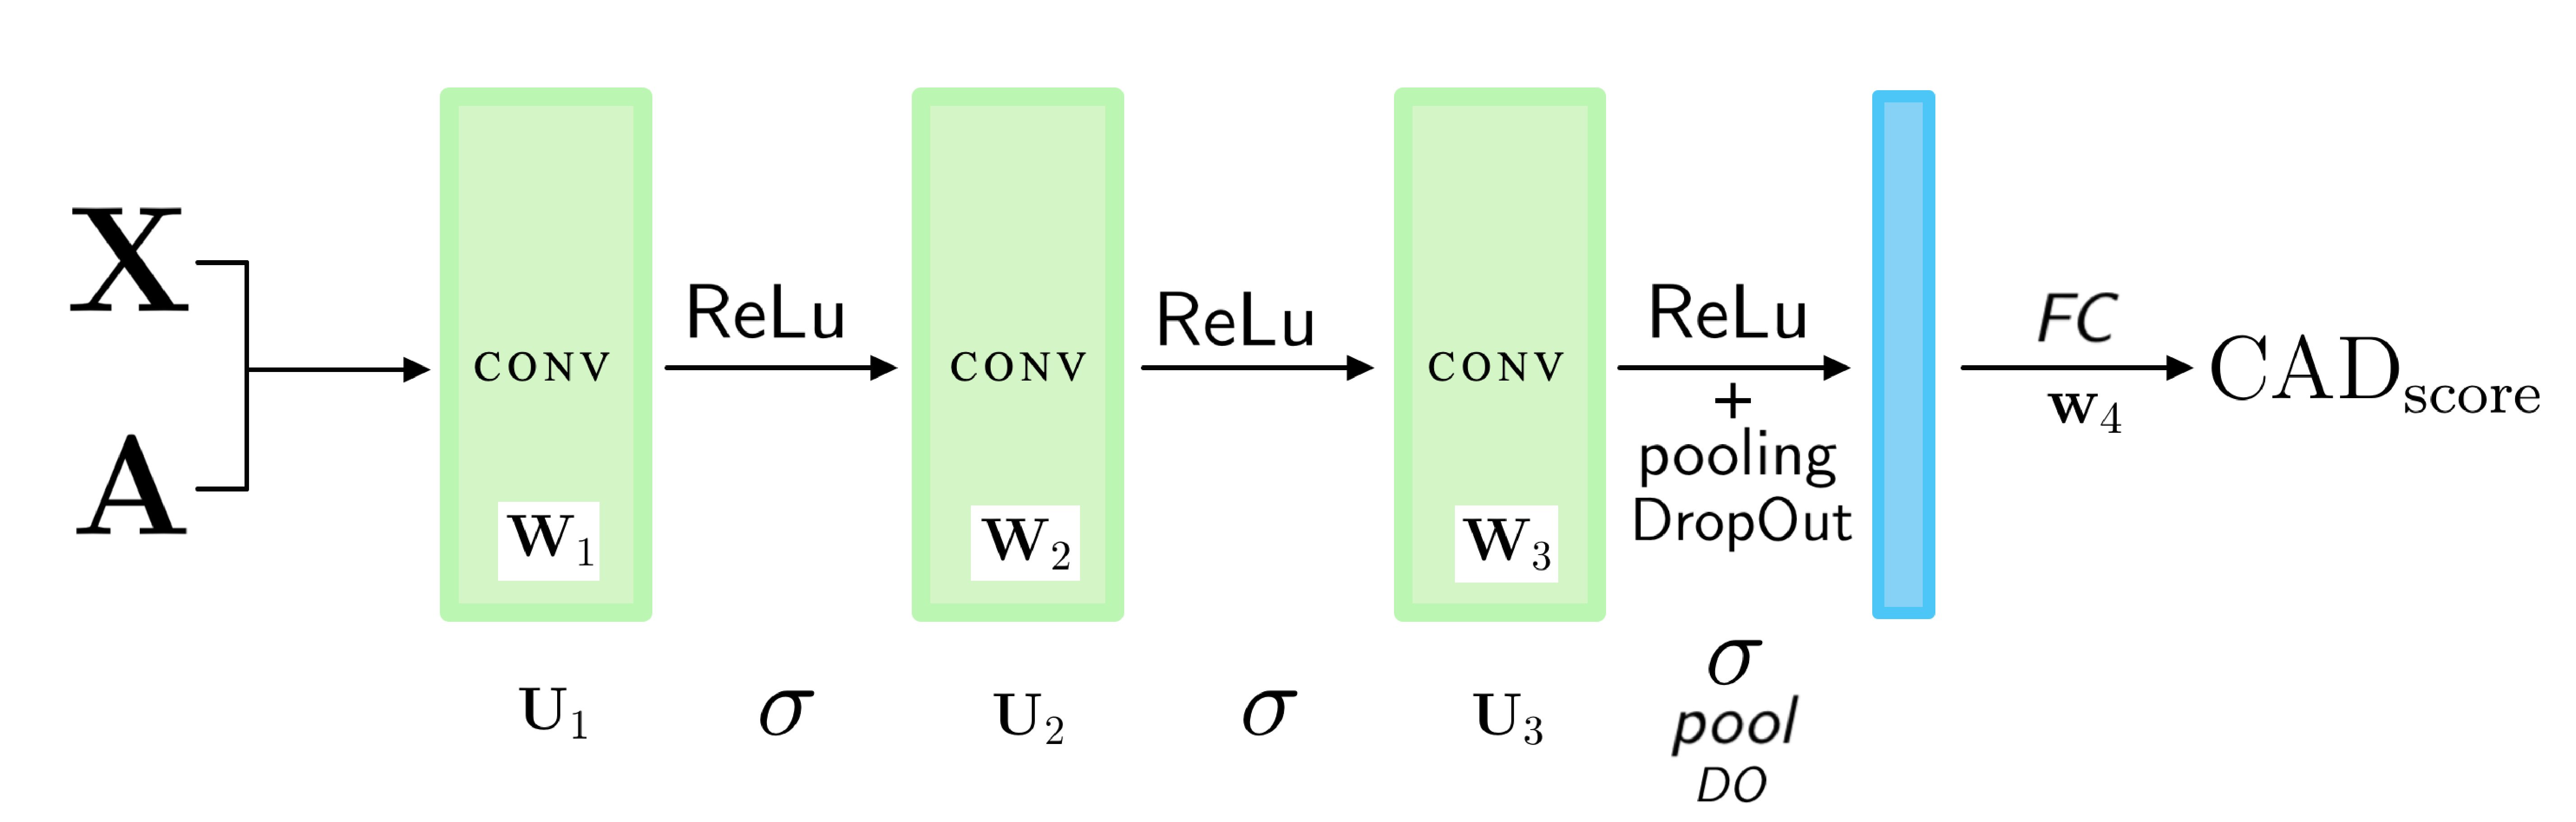
\includegraphics[width=0.9\textwidth]{net.pdf}
	\caption{Schematic representation of the architecture of the SpectralQA graph convolutional neural network used in this paper}
	\label{fig:scheme}
\end{figure}
Thus, the transformation $f: \mathbf{X} \rightarrow \text{CAD}_\text{score}$ of the resulting neural network is
\begin{align}
f = \langle \mathbf{w}_4, \text{DO} \circ \text{pool} \circ \sigma \left(\mathbf{U}_3\right) \circ\sigma\left( \mathbf{U}_2\right)\circ\sigma\left( \mathbf{U}_1\right)\rangle,
\label{regression_function}
\end{align}
where $\mathbf{U}_k= \tilde{\mathbf{D}}^{-\frac{1}{2}} \tilde{\mathbf{A}}\tilde{\mathbf{D}}^{-\frac{1}{2}} \mathbf{X} \mathbf{W}_k$, $\text{DO}$ is dropout, $\text{pool}$ is the maximum over all nodes of the graph.

%-----------------------------------------------------------------------------------------------------
\section{Results}
\label{section:data_section}

\subsection{Protein datasets}
The data for the experiment are taken from CASP competitions of the past years: CASP9-CASP12 (table~\ref{table:student}). The data consist of pairs of target and modeled structures. Each structure is described by the coordinates and chemical properties of the atoms in the structure. The regerssion model~\eqref{regression_function} is trained on the data CASP9-CASP11, tested on CASP12. For training and testing procedures, we compute $\text{CAD}_\text{score}$ using~\eqref{CAD_score} for all modeled structures based on target structures.

\begin{table}[H]
	\centering
	\caption{Datasets of protein structures}
	\begin{tabular}{p{28mm}|p{26mm}p{26mm}|p{28mm}}
		\hline Dataset & Target structures & Modeled structures& Split\\
		\hline 
		%CASP 7 & 95 & 24183 & \\
		%CASP 8 & 123 & 36176 &  \multirow{2}{*}{Train,} \\
		CASP 9 & 117 & 35963 &  \multirow{2}{*}{Train,} \\
		CASP 10 & 103 & 15450 & \multirow{2}{*}{Validation} \\
		CASP 11 & 84 & 12291 &  \\
		\hline 
		CASP 12 & 37 & 5501 & {Test} \\
		\hline
		Total & 341 & 69205 &
	\end{tabular}
	\label{table:student}
\end{table}


%-----------------------------------------------------------------------------------------------------
\subsection{Eigenspace of the adjacency matrices}

We perform a singular value decomposition for each adjacency matrix $\textbf{A}$ and the matrix after the convolution $\textbf{U}_k$ to obtain the eigenvalues of the matrices. Fig~\ref{A_eigens} and~\ref{u_k_eigens} show the eigenvalues for the modeled STRINGS\_TS3 structure of the target T0759.

\begin{figure}[H]
	\begin{minipage}[b]{0.49\textwidth}
		\centering
		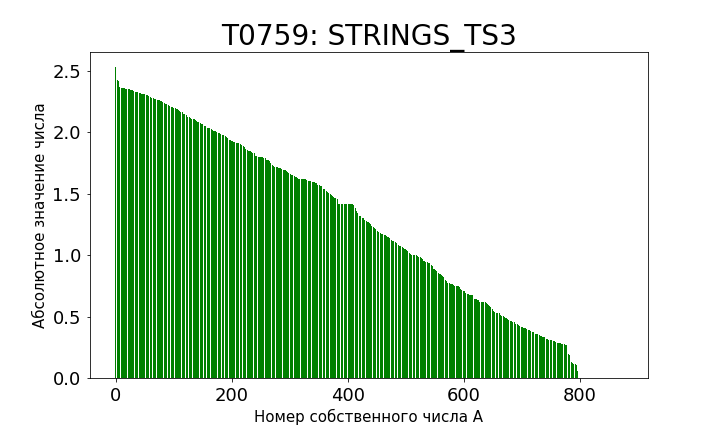
\includegraphics[width=0.85\textwidth]{T0759_A_before_conv.pdf}
		\caption{The eigenvalues of the $\textbf{A}$}
		\label{A_eigens}
	\end{minipage}
	\hfill
	\begin{minipage}[b]{0.49\textwidth}
		\centering
		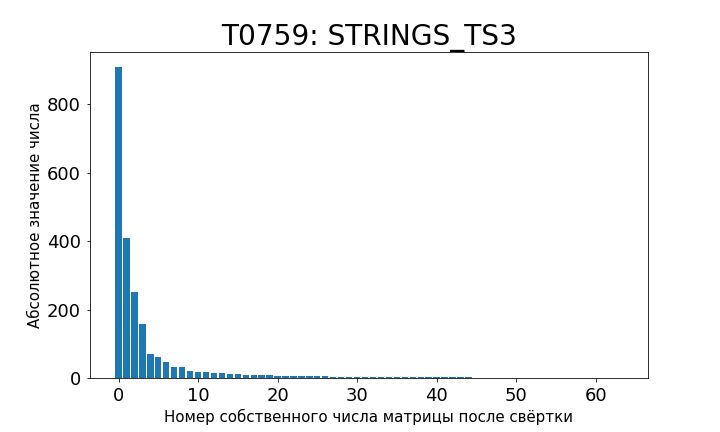
\includegraphics[width=0.85\textwidth]{T0759_X_after_conv.pdf}
		\caption{The eigenvalues of the $\textbf{U}_k$}
		\label{u_k_eigens}
	\end{minipage}
\end{figure}

The Broken stick model~\cite{Component_retention} is used to estimate the dimension of the matrix's eigenspace. The set of eigenvalues is compared with the thresholds: with the threshold A for a matrix $\textbf{A}$, with the threshold U for a matrix $\textbf{U}_k$. The $j$-th eigenvector $\textbf{A}$ is saved in the list of principal components if $\lambda_j>A$. The same is done for a matrix $\textbf{U}_k$ with the threshold U.

One modeled structure was selected at random for each target structure from the CASP11 and CASP12 datasets. 
We calculated eigenvalues for the matrices $\textbf{A}$ and $\textbf{U}_k $ for each of the selected modeled structures. The dimension of the eigenspaces of matrices is the number of eigenvalues larger than the threshold. The thresholds $U = 10$ and $A \in \{0.5, 1.0, 2.0 \} $ were considered.

The results are shown in Fig.~\ref{eigens_dims}. Each point in the figure corresponds to one modeled structure. The dimension of the eigenspace of the matrix after passing through the convolution is compressed 50-100 times. This can be explained by the strong sparseness of the adjacency matrices of protein structures.

\begin{figure}[H]
	\centering
	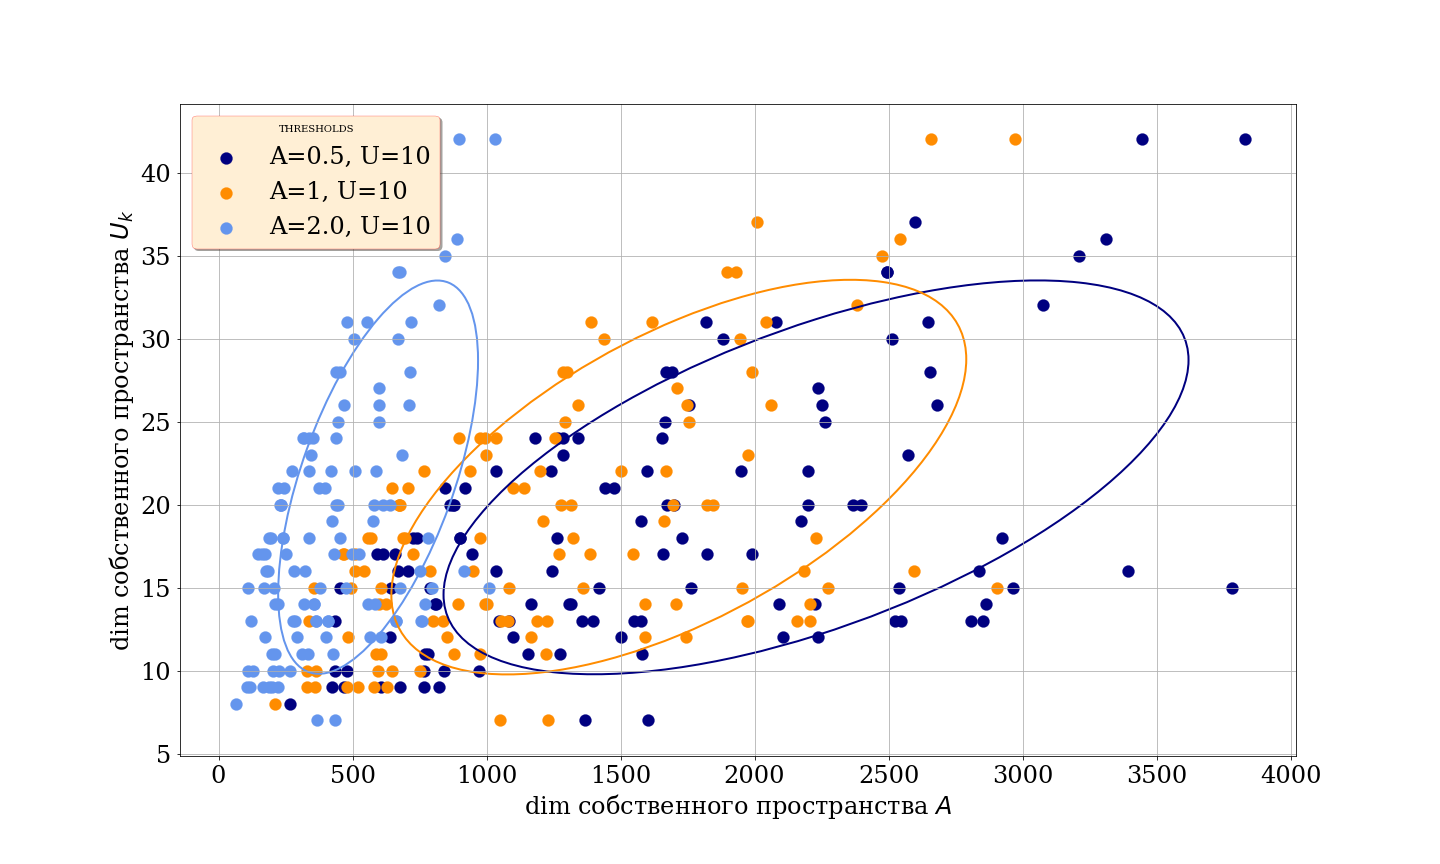
\includegraphics[width=0.73\textwidth]{eigens.pdf}
	\caption{Eigenspaces for the thresholds $U=10$ and $A~\in~\{0.5, 1.0, 2.0\}$.}
	\label{eigens_dims}
\end{figure}


%-----------------------------------------------------------------------------------------------------
\subsection{Pearson and Spearman Correlation Analysis}
The averaged over $T$ target structures Pearson~\eqref{pearson} and Spearman~\eqref{spearman}  correlation coefficients are analyzed when training a neural network. The learning process is presented in the figures~\ref{fig:GCN} и~\ref{fig:correlation}

\begin{figure}[H]
	\centering
	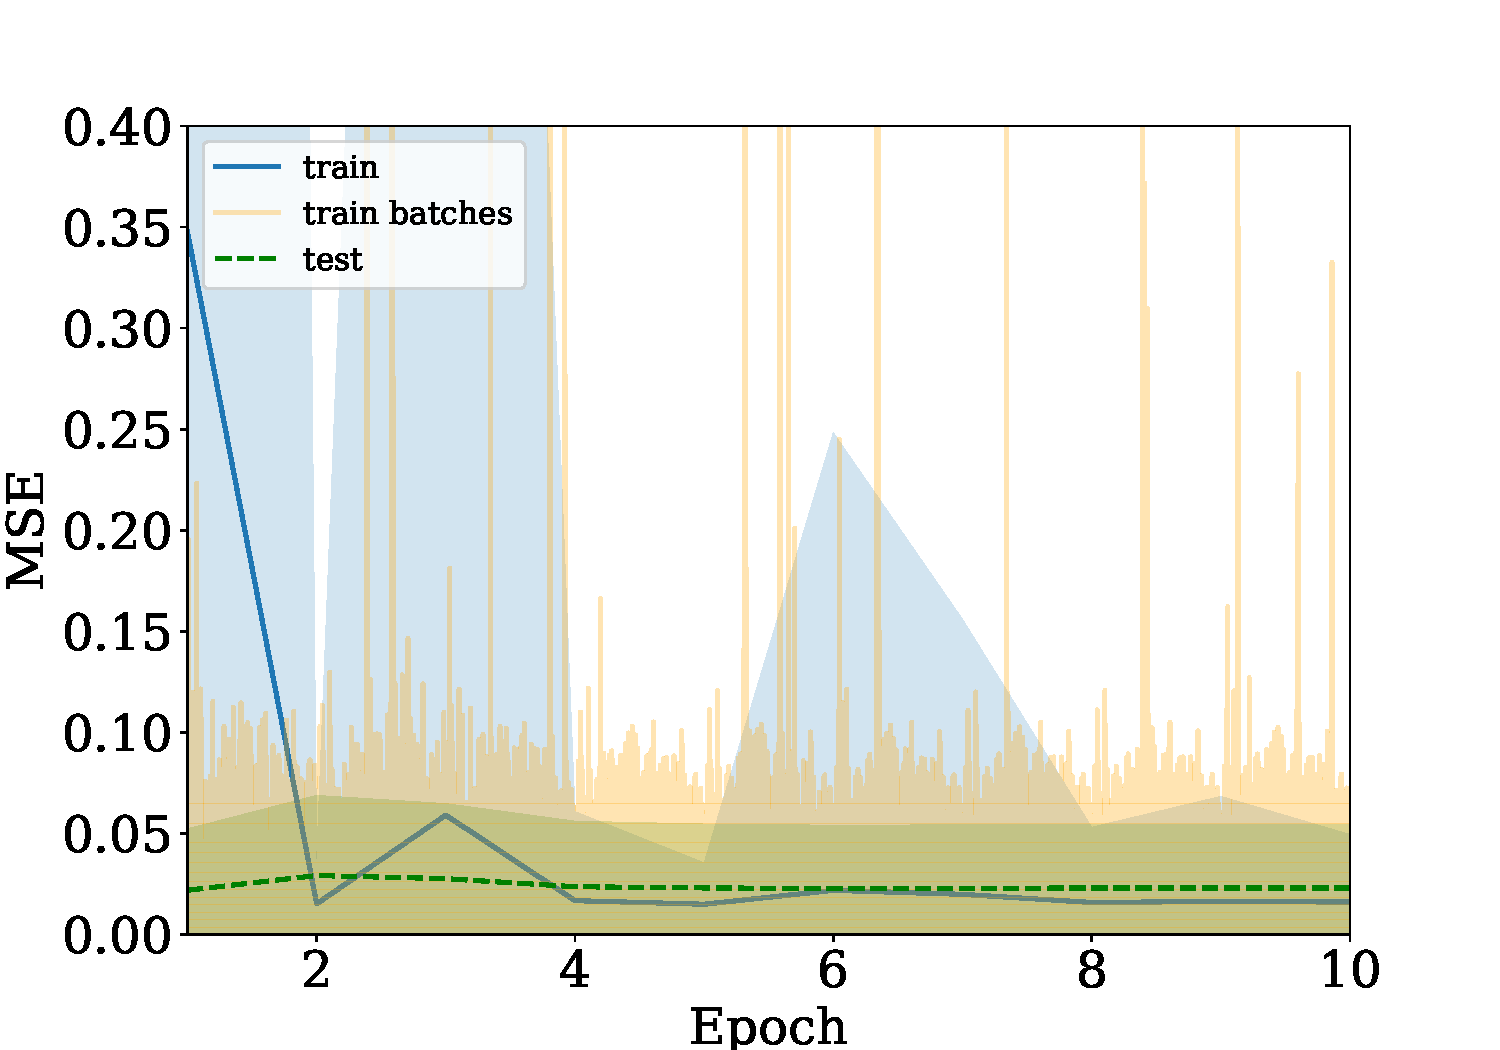
\includegraphics[width=0.6\textwidth]{training_smallset.pdf}
	\caption{MSE error plot of SpectralQA on training and test sets}
	\label{fig:GCN}
\end{figure}
The Pearson and Spearman correlation plots stabilize around one value (Figure~\ref{fig:correlation}). The large variance is explained by the fact that there are a lot of modeled structures with very low $\text{CAD}_\text{score}$ for some target structures in the data. The $\text{CAD}_\text{score}$ value will be equal or very close to 0 for poorly modeled structures due to the expression~\eqref{CAD_score}. This also explains the low value of the averaged correlation.
\begin{figure}[h]
	\centering
	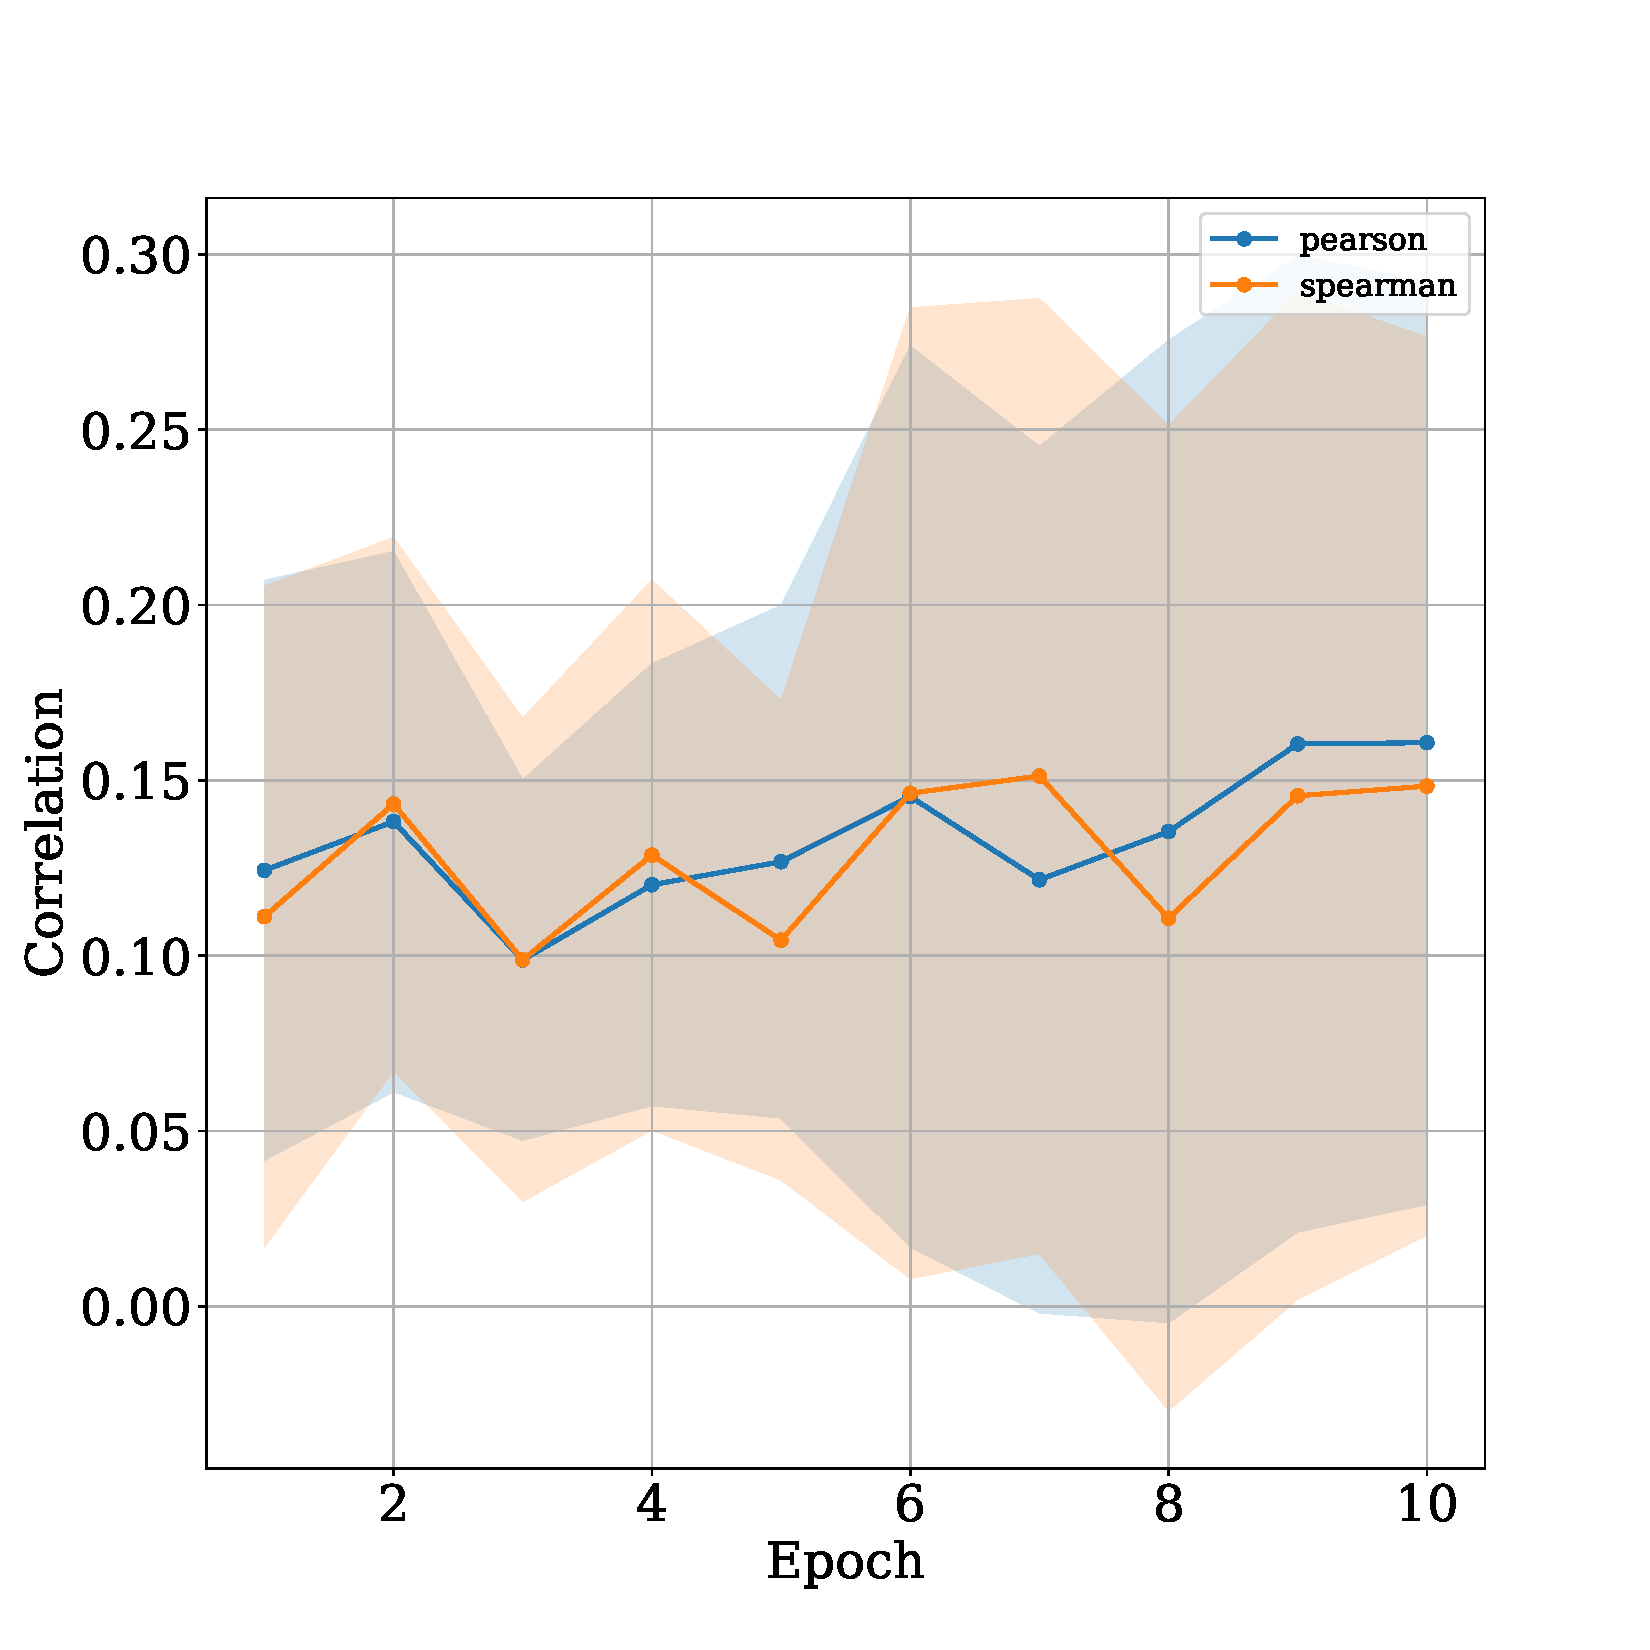
\includegraphics[width=0.5\textwidth]{training_correlations_smallsettt.pdf}
	\caption{Pearson and Spearman correlation during training procedure}
	\label{fig:correlation}
\end{figure}

Table~\ref{Tab:results} shows the results of testing the model on the data of the CASP12 competition. The correlation here is taken between all predictions and ground truth values. It can be seen from the table that the model from this paper gives a quality comparable to the quality of alternative models that give the best quality in the task.

\begin{center}
	\begin{table}[H]
		\centering
		\caption{Comparison of Pearson and Spearman correlations on CASP12 dataset of existing modern algorithms with SpectralQA model}
		%\begin{tabular}{l|l|l|l}
		\begin{tabular}{ccc}
			\hline Method & Spearmann $\rho$ &  Pearson $R$ \\
			\hline ProQ3D & 0.801 & 0.750 \\
			VoroMQA & 0.803 & 0.766  \\
			SBROD & 0.685 & 0.762  \\
			Ornate & \textbf{0.828} & \textbf{0.781}   \\
			\textbf{SpectralQA} (this paper) &   {0.746}&   0.647   \\
			\hline 
		\end{tabular}
		\label{Tab:results}
	\end{table}
\end{center}

%-----------------------------------------------------------------------------------------------------
\section{Conclusion}
In this work, we proposed a solution to the quality assessment of protein structure prediction problem using graph convolutions. The exhaustive analysis of graph convolutions on this problem and analysis of the Pearson and Spearman correlations were carried out.The quality achieved by the proposed model is comparable to the quality of alternative models that do not use graph representation of protein structures. In further studies, we plan to use other existing improvements in spectral convolutions (CayleyNet, Adaptive Graph Convolution Network) as the basis of the network architectures. It is also proposed to take into account in the data the additional chemical properties of atoms and to take into account in the adjacency matrix not only the presence of a bond, but also the distance between atoms in the presence of a bond.


%-----------------------------------------------------------------------------------------------------
% References
\bibliographystyle{ugost2008}
\bibliography{references}
\nocite{*}
	
\end{document}
